\documentclass[11pt]{article}

% Paquetes
%===================================================================================================

% Paquete para incluir codigo
\usepackage{listings}

% Paquete para incluir imagenes
\usepackage{graphicx}
\graphicspath{ {./Imagenes/} }

% Para fijar las imagenes en la posicion deseada
\usepackage{float}

% Para que el codigo acepte caracteres en utf8
\lstset{literate=
  {á}{{\'a}}1 {é}{{\'e}}1 {í}{{\'i}}1 {ó}{{\'o}}1 {ú}{{\'u}}1
  {Á}{{\'A}}1 {É}{{\'E}}1 {Í}{{\'I}}1 {Ó}{{\'O}}1 {Ú}{{\'U}}1
  {à}{{\`a}}1 {è}{{\`e}}1 {ì}{{\`i}}1 {ò}{{\`o}}1 {ù}{{\`u}}1
  {À}{{\`A}}1 {È}{{\'E}}1 {Ì}{{\`I}}1 {Ò}{{\`O}}1 {Ù}{{\`U}}1
  {ä}{{\"a}}1 {ë}{{\"e}}1 {ï}{{\"i}}1 {ö}{{\"o}}1 {ü}{{\"u}}1
  {Ä}{{\"A}}1 {Ë}{{\"E}}1 {Ï}{{\"I}}1 {Ö}{{\"O}}1 {Ü}{{\"U}}1
  {â}{{\^a}}1 {ê}{{\^e}}1 {î}{{\^i}}1 {ô}{{\^o}}1 {û}{{\^u}}1
  {Â}{{\^A}}1 {Ê}{{\^E}}1 {Î}{{\^I}}1 {Ô}{{\^O}}1 {Û}{{\^U}}1
  {ã}{{\~a}}1 {ẽ}{{\~e}}1 {ĩ}{{\~i}}1 {õ}{{\~o}}1 {ũ}{{\~u}}1
  {Ã}{{\~A}}1 {Ẽ}{{\~E}}1 {Ĩ}{{\~I}}1 {Õ}{{\~O}}1 {Ũ}{{\~U}}1
  {œ}{{\oe}}1 {Œ}{{\OE}}1 {æ}{{\ae}}1 {Æ}{{\AE}}1 {ß}{{\ss}}1
  {ű}{{\H{u}}}1 {Ű}{{\H{U}}}1 {ő}{{\H{o}}}1 {Ő}{{\H{O}}}1
  {ç}{{\c c}}1 {Ç}{{\c C}}1 {ø}{{\o}}1 {å}{{\r a}}1 {Å}{{\r A}}1
  {€}{{\euro}}1 {£}{{\pounds}}1 {«}{{\guillemotleft}}1
  {»}{{\guillemotright}}1 {ñ}{{\~n}}1 {Ñ}{{\~N}}1 {¿}{{?`}}1 {¡}{{!`}}1
}

% Para que los metadatos que escribe latex esten en español
\usepackage[spanish]{babel}

% Para la bibliografia
% Sin esto, los enlaces de la bibliografia dan un error de compilacion
\usepackage{url}

% Metadatos del documento
%===================================================================================================
\title{
    {Aprendizaje Automático - Segunda Práctica}\\
    {Complejidad de $H$ y el ruido}\\
    {Modelos Lineales}
}

\author{
    {Sergio Quijano Rey - 72103503k}\\
    {4º Doble Grado Ingeniería Informática y Matemáticas}\\
    {sergioquijano@correo.ugr.es}
}

\date{\today}

% Separacion entre parrafos
\setlength{\parskip}{1em}


% Contenido del documento
%===================================================================================================
\begin{document}

% Portada del documento
\maketitle
\pagebreak

% Indice de contenidos
\tableofcontents
\pagebreak

\section{Ejercicio 1 - Sobre la complejidad de $H$ el ruido}

\subsection{Observaciones iniciales}

Para este primer ejercicio, hacemos uso de tres funciones que se nos dan en el fichero \lstinline{template_trabajo2.py}. Las dos primeras funciones devuelven una lista de $N$ vectores de una dimensión dada.

\begin{itemize}
    \item \lstinline{simula_unif}: genera una lista de $N$ vectores aleatorios de una dimensión dada. La distribución aleatoria que siguen es una distribución uniforme en un intervalo dado
    \item \lstinline{simula_gauss}: genera una lista de $N$ vectores aleatorios de dimensión dada. La distribución aleatoria es una normal de media cero y varianza dada
    \item \lstinline{simula_recta}: genera una recta aleatoria que pasa a través de un intervalo 2-dimensional dado
\end{itemize}

Además, al principio de cada función asociada a los ejercicios (\lstinline{ejercicio1()}, \lstinline{ejercicio2()}, \lstinline{ejercicio_bonus()}) establecemos una semilla aleatoria fija con la orden \lstinline{np.random.seed(123456789)}. Así, los resultados que obtenemos serán reproducibles. Aunque por estar usando probablemente distintos configuraciones de sistemas operativos, hardware, versión de \lstinline{python}, \ldots, los resultados obtenidos por los profesores de prácticas no serán exactamente los mismos cuando exista un factor aleatorio.

\subsection{Apartado 1}

En este apartado se pide que dibujemos las nubes de puntos simuladas con las dos primeras funciones dadas por los profesores. Para ello empleamos los siguientes parámetros:

\begin{itemize}
    \item $N = 50$
    \item $dim = 2$
    \item $rango = [-50, 50]$
    \item $\sigma = [5, 7]$ donde $\sigma$ indica la varianza (por tanto sería más adecuada la notación $\sigma^2$) en el eje $x$ e $y$
\end{itemize}

Lanzando el código obtenemos las dos siguientes nubes de puntos:

\begin{figure}[h]
    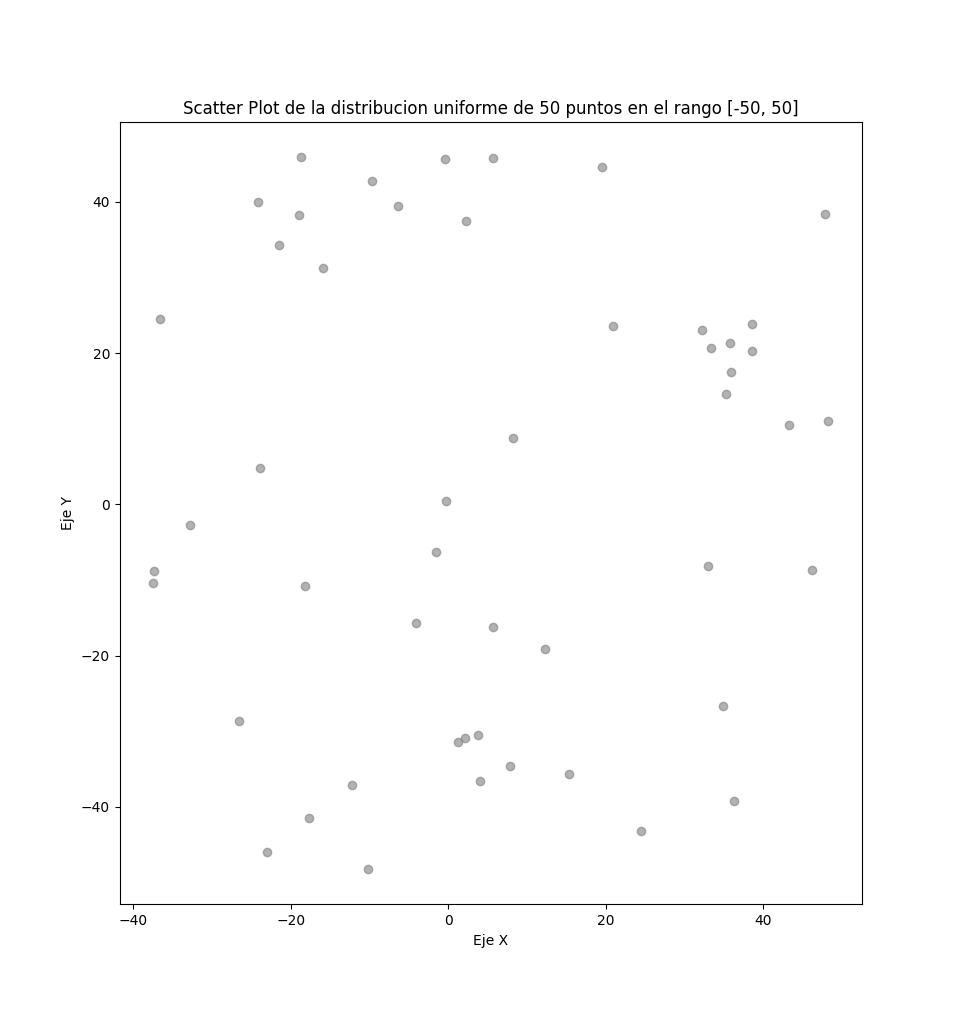
\includegraphics[width=0.60 \textwidth]{nube_puntos_uniforme}
    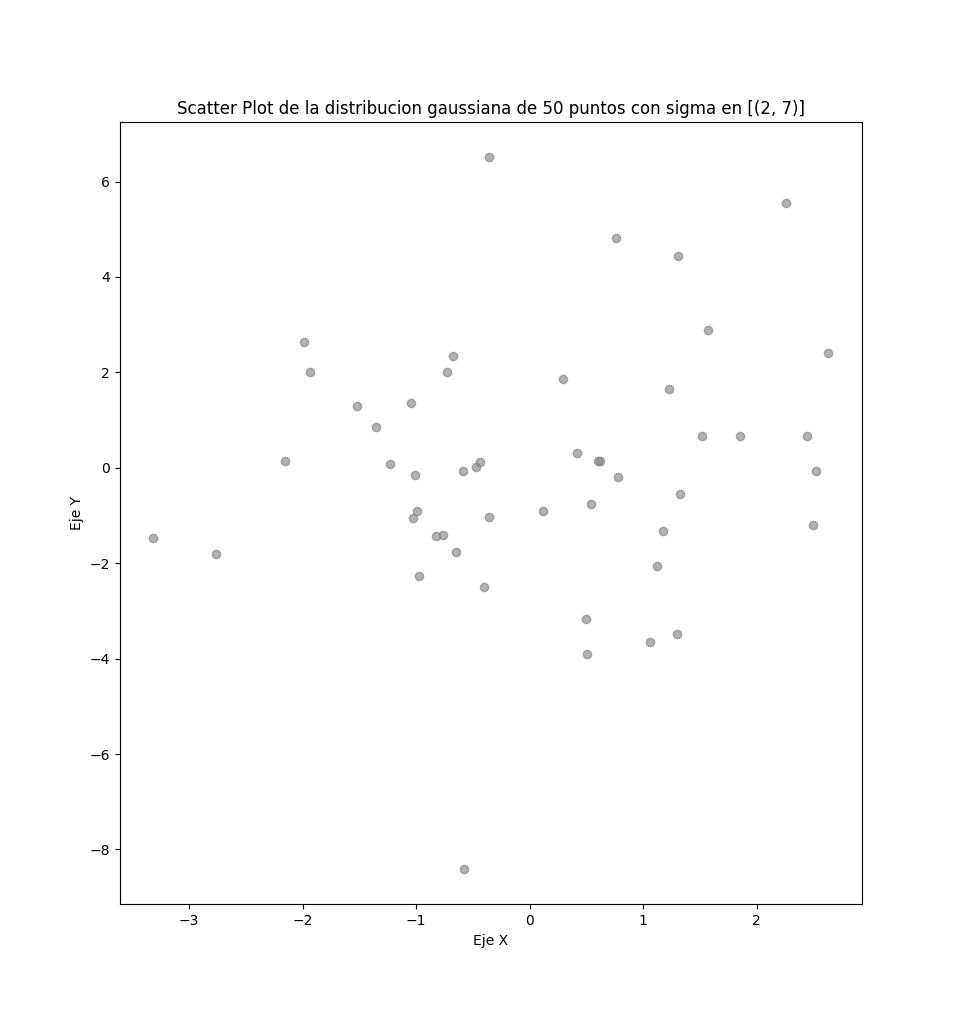
\includegraphics[width=0.60 \textwidth]{nube_puntos_normal}
    \caption{Nubes de puntos de las dos distribuciones}
\end{figure}

\subsection{Apartado 2}

Vamos a valorar la influencia del ruido en la selección dela complejidad de la clase de funciones. Para ello generamos una muestra de puntos bidimensionales. En concreto, generamos 100 puntos en el intervalo $[-50, 50]$.

Una vez que generamos esta muestra de datos, los etiquetamos usando una recta generada aleatoriamente, usando la función dada por los profesores \lstinline{simula_recta}. Con la recta $f(x) = ax + b$, etiquetamos los datos con la función de etiquetado $(x, y) \rightarrow sign(y - ax - b)$. Esta función toma un punto $x, y$, calcula su distancia a la recta $f$ (que se corresponde con $y - f(x)$) y como etiqueta asigna el signo de esta distancia. Es decir, estamos mirando si un punto se queda por encima de la recta (etiqueta $+1$) o por debajo (etiqueta $-1$).

\subsubsection{Subapartado a)}

El enunciado de este apartado especifica que se vuelva a generar la muestra de datos, como se especifica anteriormente. Por tanto, se puede ver que la nube de datos no es la misma que la nube de datos uniforme del Apartado 1.

La gráfica de los datos etiquetados, junto a la recta que se usa para etiquetar, es la siguiente:

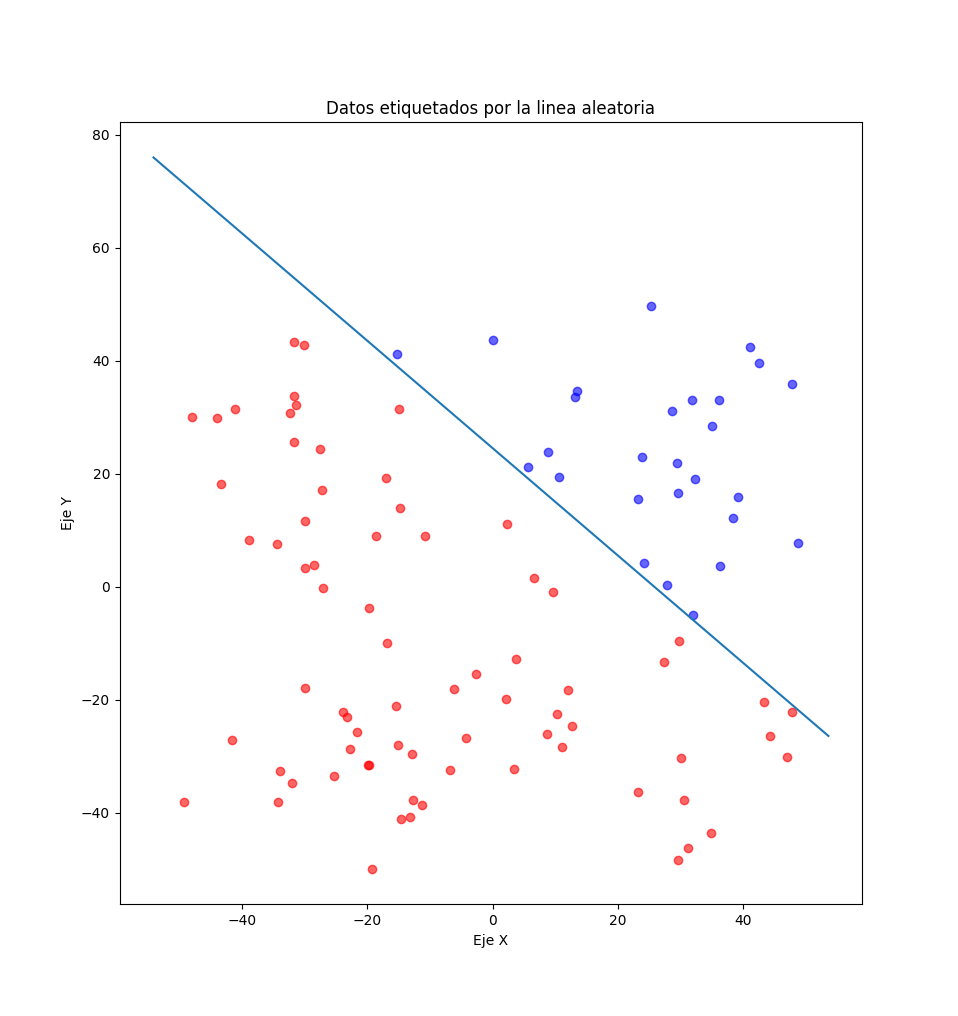
\includegraphics[width=0.9 \textwidth]{puntos_clasificados_recta01}

La gráfica deja claro que los puntos han sido correctamente clasificados a partir de la recta generada aleatoriamente.

\subsubsection{Subapartado b)}

Modificamos el 10\% de las etiquetas positivas y un 10\% de las etiquetas negativas, y volvemos a mostrar la gráfica.

Para realizar esto de forma eficiente, lo que hacemos es tomar dos vectores, uno con las posiciones de etiquetas positivas y otro con las posiciones de las etiquetas negativas. Calculamos el número de etiquetas de cada tipo a cambiar ($N_1, N_2$), a partir de un porcentaje arbitrario (para nuestro caso concreto, usamos $0.1$). Hacemos un \emph{shuffle} de los dos vectores de posiciones y cambiamos el etiquetado de las $N_1$ y $N_2$ primeras posiciones del vector remezclado. Con ello modificamos un porcentaje dado de las etiquetas de forma aleatoria. Todo esto se puede ver en la función \lstinline{change_labels}.

Notar que podemos tener clases sin puntos. Es decir, que no etiquetamos ningún dato con o bien $+1$ o bien $-1$. En el caso de la recta, es muy improbable que esto pase. Pero en el siguiente subapartado, con ciertas funciones es muy probable que pase.

El gráfico de clasificación tras esta modificación aleatoria es:

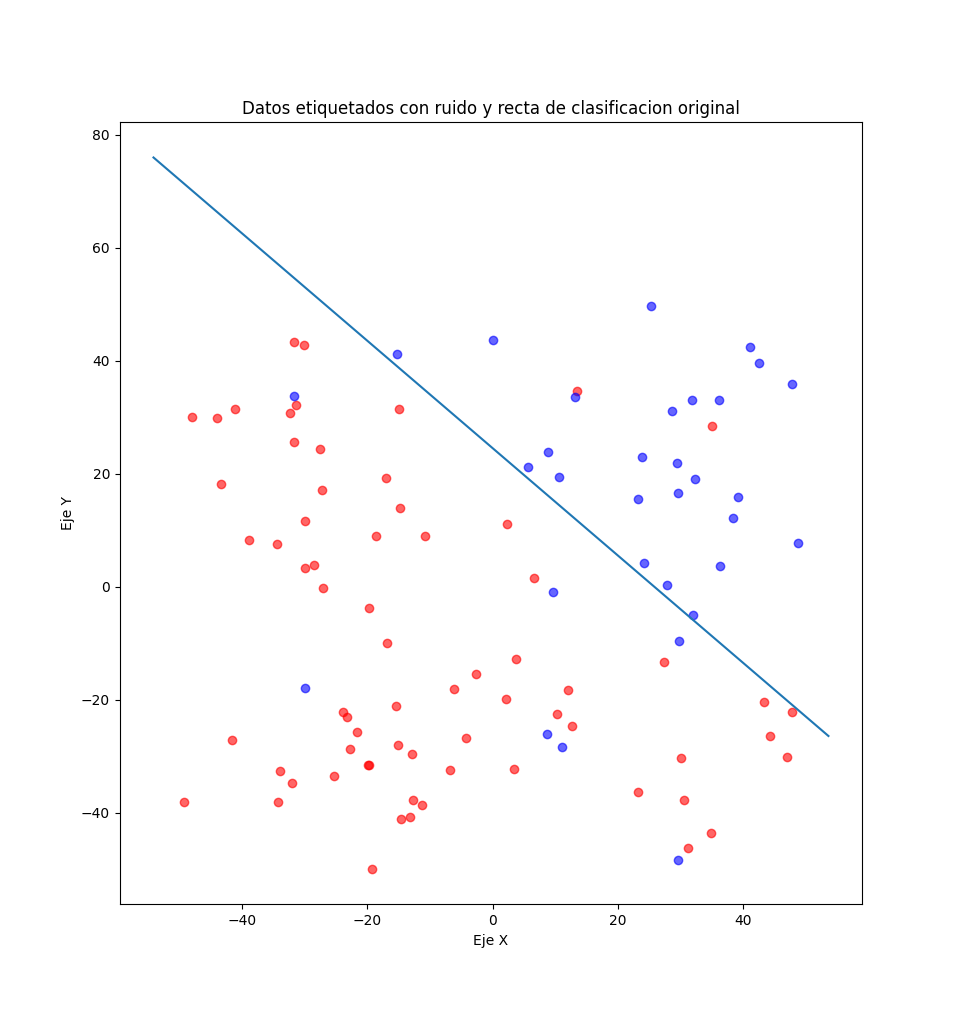
\includegraphics[width = 0.8 \textwidth]{puntos_clasificados_recta_aleatorizados01}

Se ve con claridad cómo esta operación introduce ruido sobre nuestras etiquetas.

\subsubsection{Subapartado c)}

Consideramos ahora las siguientes funciones que definen una frontera de clasificación:

\begin{itemize}
    \item $f_0(x, y):= (x - 10)^2 + (y - 20)^2 - 400$
    \item $f_1(x, y):= \frac{1}{2} (x + 10)^2 + (y - 20)^2 - 400$
    \item $f_2(x, y):= \frac{1}{2} (x - 10)^2 - (y + 20)^2 - 400$
    \item $f_3(x, y):= y - 20x^2 -5x +3$
\end{itemize}

Usamos estas funciones de frontera para clasificar los datos generados en el Subapartado a). También modificamos un 10\% de las etiquetas positivas y negativas aleatoriamente. Además, mostramos las regiones de clasificado positivo y negativo de las funciones empleadas.

Con las funciones de frontera $f_i(x, y)$, realizamos el etiquetado de forma análoga que con la recta, etiquetando con el valor $sign(f_i(x,y))$.

Podríamos haber intentado mostras las líneas de frontera de etiquetado, como hemos hecho con la recta. Pero para ello, tenemos que calcular un despeje de $f(x, y)$, o bien de $x$ o bien de $y$, pues $f(x, y)$ viene dada de forma implícita. No todas las funciones tienen un despeje global, por lo que habría que emplear el teorema de la función implícita para realizar despejes locales, y después concatenar las graficas obtenidas con los despejes locales. Hemos considerado que esto entorpecía demasiado el código. Así que la solución encontrada ha sido usar la función \lstinline{contourf} de la librería \lstinline{matplotlib.pyplot}, con la que pintaremos las regiones en las que clasificamos positivamente y las regiones en las que clasificamos negativamente.

Mostramos las gráficas obtenidas:

% TODO -- no se muestra donde quiero que se muestre
\begin{figure}[H]
    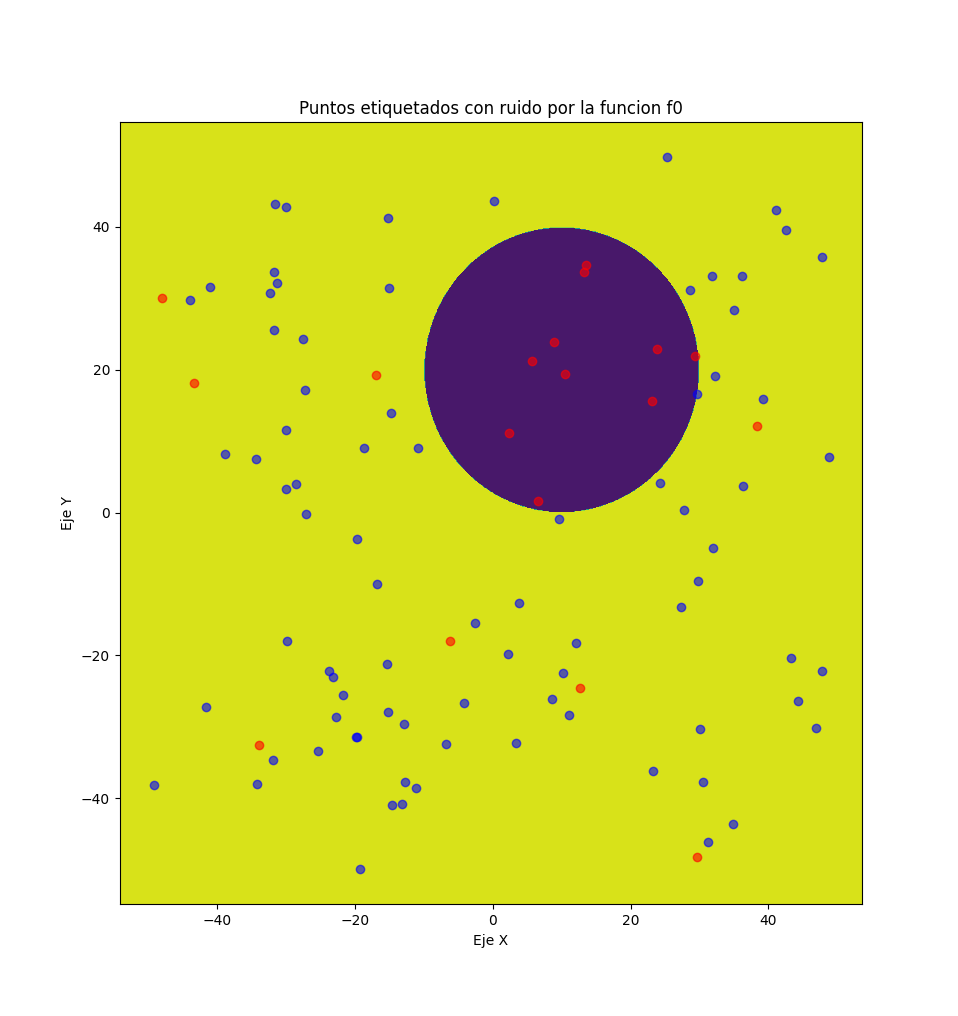
\includegraphics[width=0.60 \textwidth]{puntos_clasificados_f0.png}
    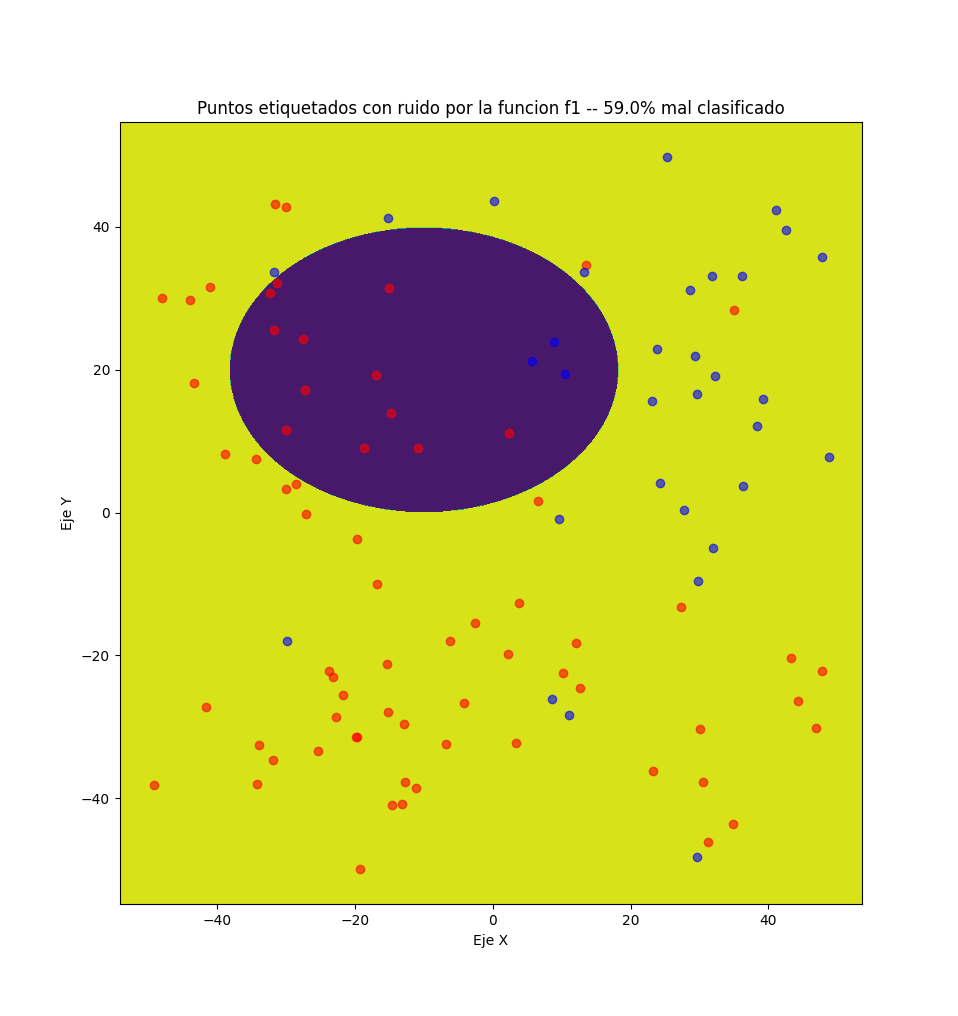
\includegraphics[width=0.60 \textwidth]{puntos_clasificados_f1.png}

    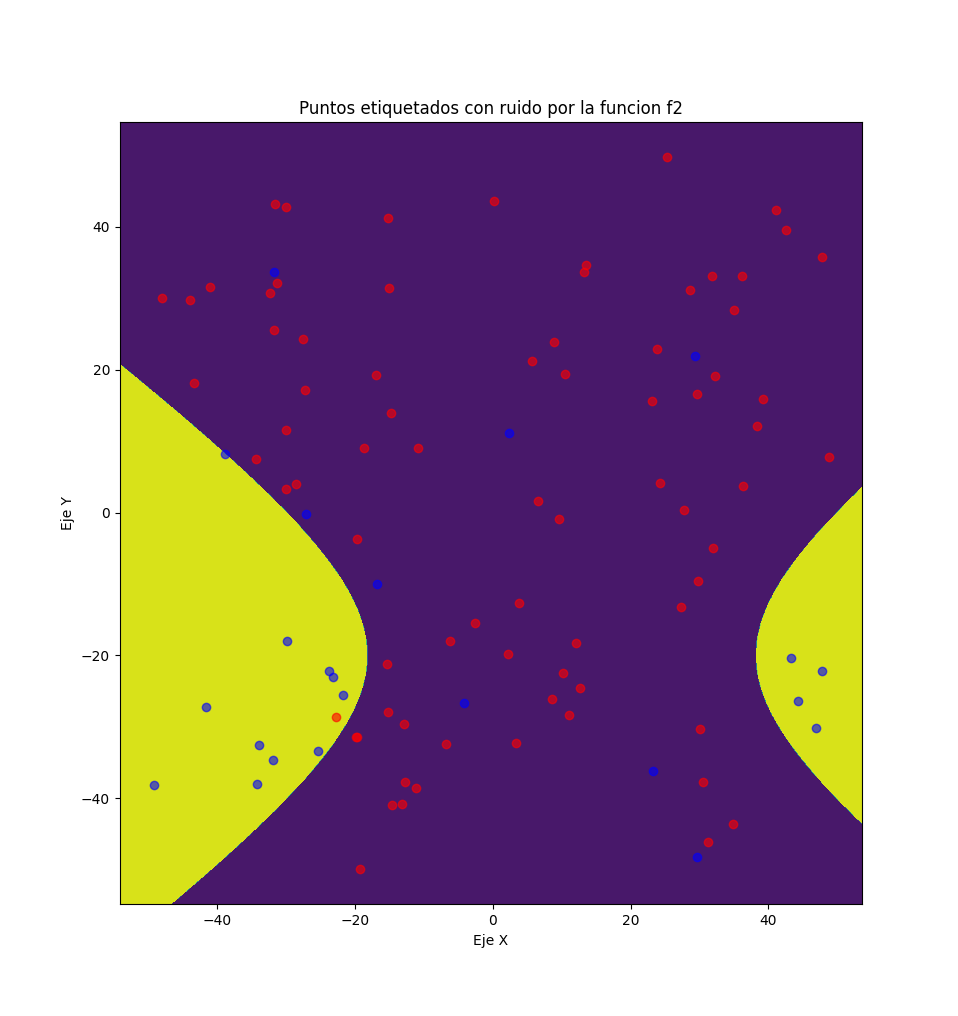
\includegraphics[width=0.60 \textwidth]{puntos_clasificados_f2.png}
    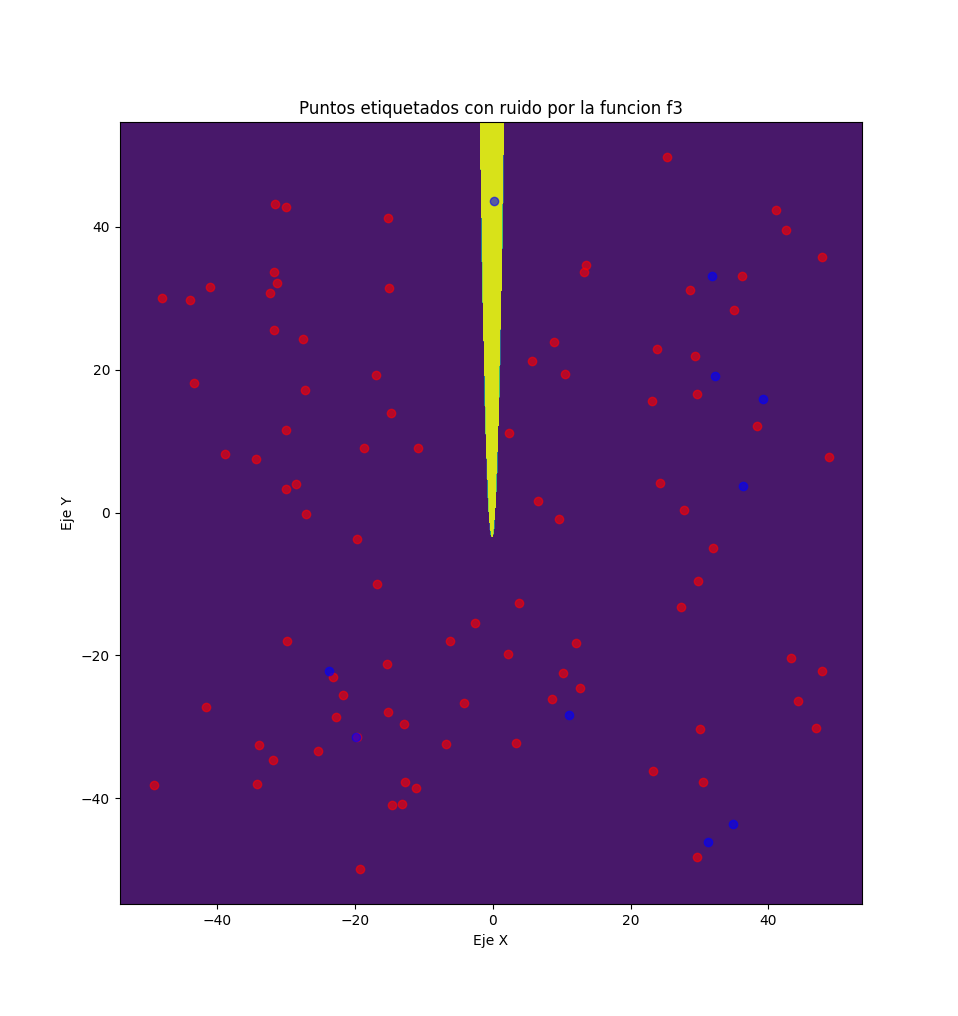
\includegraphics[width=0.60 \textwidth]{puntos_clasificados_f3.png}

    \caption{Etiquetado ruidoso con las cuatro funciones dadas}
\end{figure}

Es claro que la recta realiza una clasificación mucho más sencilla que estas nuevas funciones de clasificación, pues divide el espacio en dos regiones sencillas: la región por encima de la recta y la región por debajo de la recta. $f_0$ ya es más compleja pues estamos considerando la región fuera y dentro de un círculo, que no está centrado en el origen. $f_1$ es algo más compleja, pues ahora no consideramos un círculo, sino una elipse (añadimos un nuevo parámetro al modelo, el achatamiento del eje $x$ dado por el factor $\frac{1}{a^2}$). En $f_2$ estamos considerando regiones hiperbólicas, que viene determinada por el mismo número de parámetros que $f_1$, aunque la forma de las regiones cambie al cambiar la cónica cambiando el signo. Y en este caso, hay un predominio de región de etiquetado positivo frente a la región de etiquetado negativo. Y finalmente en $f_3$ consideramos una parábola, cuya región de etiquetado negativo tiene un área muy pequeña comparada a la región de etiquetado positivo.

Bajo estas condiciones es algo complicado comentar si estas funciones más complejas son mejores clasificadores que la función lineal, pues esto dependerá de una serie de factores:

Para empezar estamos trabajando con 100 puntos o datos. Debemos emplear algún método para concer si la complejidad de nuestras funciones se adecúa a la cantidad de datos con los que estamos trabajando. Esta herramienta será la \textbf{dimensión de Vapnik-Chervonenkis}. Sabemos que en el caso de la recta, $d_{VC} = d + 1 = 3$, y por tanto, la regla práctica para generalizar bien $N \geq 10 d_{VC}$ se cumple. Para el caso del círculo y de la elipse, tenemos también que $d_{VC} = 3$. Esto no es difícil de probar, al tener una dimensión tan baja, con ejemplos \footnotemark. Por tanto, a nivel de generalización, con los 100 datos que tenemos es suficiente pues $100 \geq 3 * 10$. Para el caso de la hipérbola y de la parábola hemos comprobado que $d_{VC} = 3$ yendo ejemplo por ejemplo (puede estar mal hecho el cálculo). Por lo cual, todas las funciones tienen una cantidad suficiente de datos acorde a $d_{VC}$ como para que no haya problemas para generalizar (siempre siguiendo la regla práctica $N \geq d_{VC} * 10$).
\footnotetext{En \cite{PowerPoi66:online} se muestra de forma visual la prueba de esto con los conjuntos dados de datos. En \cite{machinel96:online} se realiza una prueba formal de este hecho.}

Sería más adecuado realizar experimentos con un dataset de entrenamiento y otro de test para comprobar empíricamente que, efectivamente, con 100 datos no tenemos problemas de generalización.

Notar que la función lineal sigue siendo más sencilla aunque $d_{VC}$ parezca indicar lo contrario. Esto se debe a que en el análisis \emph{VC}, nos situamos en el peor de los casos, es un análisis muy pesimista.

Otro punto a tener en cuenta es el problema que estamos considerando. No tiene sentido plantearse el clasificado en abstracto y comparar lo bueno que son los clasificadores desde este punto de vista. Si las características del problema tienen un carácter lineal (al doble de ingresos, el doble de probabilidad de que nos acepten la solicitud de un crédito, por ejemplo), las funciones de clasificado no lineales no tienen demasiado sentido. Si por otro lado las características de los datos no son lineales, entonces puede tener más sentido usar clasificadores no lineales a pesar de que representen un modelo más complejo, pues serían más correctos desde la perspectiva del problema a resolver.

Respecto al proceso de modificación de etiquetas, las condiciones en la que hemos realizado este proceso también complica algo las cosas. Hemos modificado, aleatoriamente, un 10\% de las etiquetas positivas y otro 10\% de las etiquetas negativas. En este proceso da bastante igual la forma que tome $f$. En el sentido en el que, podemos pensar que la recta es muy robusta frente al ruido, o más robusta que una elipse. Pero a la hora de ejecutar el cambio aleatorio, esto no se tiene en cuenta.

Sin embargo, si que hemos detectado una característica en la que la forma de $f$ influye en el proceso. Esto se ve claro con $f_3$. Al tener una región mucho más pequeña que la contraria (en este caso, región de etiquetado negativo mucho más pequeña que la región de etiqetado positivo), es muy probable que no hayamos clasificado ningún punto como negativo, y por tanto realizamos modificaciones del tipo $negativo \rightarrow positivo$, solo modificaciones del tipo $positivo \rightarrow negativo$. Aún así, esto no es demasiado relevante

Así queda justificado que el proceso de introducción de ruido no es muy informativo. Un proceso de introducción de ruido mucho más interesante podría haber sido seleccionar aleatoriamente un porcentaje de las etiquetas, tanto positivas como negativas, y en vez de cambiar arbitrariamente su etiqueta, modificar en un cierto rango acotado su posición, y ver si en esa nueva posición se etiquetaría con el otro valor.

Esto nos daría más información sobre la robustez de nuestro clasificador frente al ruido. Por ejemplo, en el caso de la recta, un punto alejado de la frontera no cambiaría de etiqueta (con un rango de variación de coordenadas razonable), mientras que un punto muy cercano a la frontera sí que cambiaría. Como se puede ver en la imagen, la mayoría de puntos no se encuentran muy pegados a la frontera. Por otro lado, considerando $f_3$, podríamos pensar que todos los puntos de etiquetado negativo se saldrían de la región de etiquetado negativo, al ser esta muy estrecha, concluyendo que el clasificador es muy frágil frente al ruido.

Otra forma de medir esta \emph{robustez} sería calcular la longitud de las fronteras de nuestro clasificador. A mayor longitud, tenemos un modelo más complejo, que es más probable de sobreajustar. Además, a mayor longitud es más probable que un cambio de coordenadas aleatoria, anteriormente discutida, provoque un cambio de etiqueta. Y por tanto es más probable que el ruido afecte a nuestro problema.

Resumiendo, consideramos insuficiente la información dada para comparar las funciones de clasificación. Por tanto, realizamos nuevas consideraciones para tratar de realizar un mejor análisis, y proponemos una forma sintética de introducir ruido que pensamos que puede ser más adecuada a la hora de analizar la robustez de los clasificadores frente al ruido.



\pagebreak


% Bibliografia
\bibliography{References}
\bibliographystyle{ieeetr}

\end{document}
